\begin{Exercise}[title=Goutte de pluie et pare brise]
  On pose un objet ponctuel de masse m sans vitesse initiale, à l'angle
  $\theta_0$ sur un support circulaire de rayon $R$, se déplaçant horizontalement
  dans le champ de pesanteur uniforme, avec une accélération
  constante $\gamma_0$. On négligera les frottements dans un premier temps.
  \begin{center}
    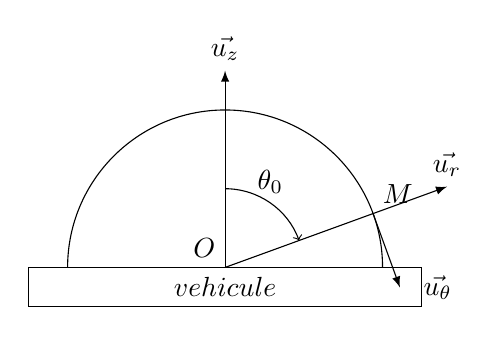
\begin{tikzpicture}
      \draw (2,0) arc (0:180:2);
      \draw (-2.5,-.5) rectangle (2.5,0) node[pos=.5] {$vehicule$};
      \draw [->,>=latex] (0,0) -- (0,2.5) node[above]{$\vec{u_z}$};
      \draw (0,0) node[above left]{$O$} -- (20:2) node[above right] {$M$};
      \draw[->,>=latex] (20:2) -- ++(20:1) node[above]{$\vec{u_r}$};
      \draw[->,>=latex] (20:2) -- ++(-70:1) node[right=5pt]{$\vec{u_\theta}$};
      \draw[->] (0,1) arc (90:20:1) node [midway, above]{$\theta_0$};
    \end{tikzpicture}
  \end{center}
  \Question Position(s) d'équilibre et stabilité de ce système ?
  \Question Pourquoi les pares brises de voitures ne sont ils pas des
  plans inclinés (ils possèdent une légère courbure?) ?
  \Question Quelles phénomènes rajoutent les frottements au problème ?

\end{Exercise}
\begin{Answer}
 2 forces le poids, et la réaction du support. un paramètre : $\theta$, selon $u_z$ ,
 le poids s'écrit $-mg$, pour la réaction du support c’est uniquement selon
 $u_r$.
  le poids se réécrit donc $-mg cos(\theta)$ selon $u_r$ et $-mg sin(\theta)$  selon $u_\theta$
 3 eme loi Newton accélération ici donnée par l'énoncé équilibre pour $\tan(\theta_{eq}) = \gamma_0/ g$
 Raisonnement énergétique à aborder à l'oral
 stabilité : montrer que si $\theta< \theta_{eq}$ alors l'objet remonte, sinon pour $\theta >
 \theta_{eq}$, l'objet redescends, instable.
 Cette instabilité favorise la disparition des gouttes de pluie.
 Qualitativement les frottements vont avoir tendance à stabiliser la position
 d'équilibre (insister sur l'importance d'avoir des essuie-glaces!)
\end{Answer}
